\chapter{The Consistency Problem in Indefinite Relations}\label{chap:consistency}
\index{Consistency Problem}
\index{NP-Complete|see{Consistency Problem}}

In this chapter we demonstrate how NDs may be applied within a
heuristic chase based algorithm for approximating solutions to the
consistency problem \cite{vn95}. We also demonstrate how resampling
may be applied in a dynamic fashion to decide upon suitable sample
sizes for the indefinite relation in question.

\medskip

In section~\ref{sec:intro} we motivate the application of indefinite
information in relations, referring to the work of
\cite{vn95,inv91,ivv95}. The consistency problem is presented in
section~\ref{sec:conprob}. Section~\ref{sec:algdes} details our
approach to the consistency problem, detailing the chase procedure for
indefinite information relations, the algorithms applied and the use
of two resampling techniques, the bootstrap and the jackknife, for
sample size determination. Section~\ref{sec:cpresults} presents the
extensive simulations conducted on randomly generated indefinite
relations, both uniform and biased with respect to indefinite cell
appearance. We also present the details of how the simulations were
assessed and the results achieved. We conclude in~\ref{sec:cp_disc}
with a discussion of further work and introduce how our work might be
extended to search for phase transistions in our approximation
technique for relations containing indefinite information.

\section{Indefinite Information in Relations}\label{sec:intro}

In section~\ref{subsec:rev_indef} we introduced the background on
indefinite information representation in relations principally
focusing on the use of $OR$-objects. We now discuss applications of
indefinite information and formalise our representation.

\subsection{Applications}
\index{Incomplete Information in Relations}
\index{Incomplete Information}
\index{Indefinite Information}
\index{OR-object}
\index{NULL value}
		
Indefinite information representation in relations has been shown to be 
a useful facility for incomplete specifications in design and planning
applications \cite{inv91,ivv95,vn95}. We define {\em indefinite cells} as cells
containing one or more values which represent a set of possibilities denoting
 the current limit of knowledge in the database. Any indefinite cell in 
column $A$ which contains the complete domain allowed for A is equivalent to
the traditional NULL value \cite{lip79}.
 A definite relation extracted from
one containing indefinite information is a relation with the same schema
and definite cells, which are invariant throughout, but with each indefinite
cell, say I, replaced with a definite cell containing one value from I.  
Associated with an indefinite
relation may be a set of integrity constraints, primarily FDs, the
most common integrity constraint in relational databases. 
\medskip


\cite{inv91} introduced OR-objects for use within design, planning and
scheduling operations, motivated by the lack of functionality in
information systems to handle
\begin{itemize}
\item coexistence of objects in different stages within the design
process
\item ability to evaluate hypothetical queries
\item to allow choice within the data model
\end{itemize}

\cite{inv91} presents difference between the interpretational and
structural levels of a schedule. In this work we proved a methodology
for assessing interpretational information content of indefinite
relations. The interpretational level refers to the final designs,
possible worlds in our interpretation, of an indefinite relation
whilst the structural levels we are concerned with the indefinite
relation itself. If we consider a structural query discussed in
\cite{inv91} such as ``are there two people in a travel relation $c$
with common destinations'' may be addressed by including NDs as
constraints within the respective data model.  \cite{inv91} formalises
views which allow for querying at either the interpretational or
structural level, or a combination of the two. The data complexity of
the query language is shown to be CoNP-complete, correlating with the
proof given in \cite{vn95} that the consistency problem is NP-complete
due to the fact that a query might ask if all schedules are invalid (a
structural query) consistent with all schedules violating an FD set.

\medskip

\cite{ivv95} extends this work by providing a complexity tailored
design methodology which restricts parameters of database design using
indefinite information so as to ensure polynomial time querying. For
example, a conjunctive query in a database over two relations remains
in PTIME if the database is restricted to having indefinite
information in only one relation.


\begin{definition}[The set of {\em possible worlds}]
\begin{rm}
The set of {\em possible} definite tuples of an indefinite tuple $t$, 
denoted by POSS($t$), is the set of tuples given by
\begin{displaymath}
\{u \mid u \mbox{ is definite and } \forall A \in R, u[A] \in t[A]\}.
\end{displaymath}
The set of {\em possible worlds}
of a relation $r = \{t_1, t_2, \ldots, t_n\}$, denoted by POSS($r$),
is the set of relations given by
\begin{displaymath}
\{s \mid s = \{u_1, u_2, ..., u_n\} \mbox{ and } 
u_1 \in {\rm POSS}(t_1), u_2 \in {\rm POSS}(t_2),
\ldots u_n \in {\rm POSS}(t_n)\}.
\end{displaymath}
 \end{rm}
\end{definition}


\begin{definition}[Satisfaction of an FD in an Indefinite Relation]\label{def:sat-indef}
\begin{rm}
Let $s \in$ POSS($r$), be a definite relation over R.
An FD X $\to$ Y is {\em satisfied} in $s$,
denoted by $s \models$ X $\to$ Y, whenever
$\forall t_1, t_2 \in$ s, if $t_1$[X] = $t_2$[X] then $t_1$[Y] = $t_2$[Y].
A set of FDs F is {\em satisfied} in $s$,
denoted by $s \models$ F, whenever
$\forall$ X $\to$ Y $\in$ F, $s \models$ X $\to$ Y.

\smallskip

A set of FDs F is {\em weakly} satisfied  
(or simply satisfied whenever no ambiguity arises) in a relation $r$,
denoted by $r \weak$ F, whenever 
$\exists s \in$ POSS($r$) such that $s \models$ F.
If $r \weak$ F we say that $r$ is {\em consistent} with respect to F 
(or simply $r$ is consistent if F is understood from context);
otherwise if $r \notweak$ F then we say that $r$ is {\em inconsistent}
with respect to F (or simply $r$ is inconsistent).
\end{rm}
\end{definition}


\begin{definition}[Satisfaction of an ND in an Indefinite Relation]\label{def:sat-nd-indef}
\begin{rm}
Let $s \in$ POSS($r$), be a definite relation over R.
An ND X $\to^k$ Y is {\em satisfied} in $s$,
denoted by $s \models$ X $\to^k$ Y, whenever
$\forall t_1, t_2, \ldots, t_k, t_{k+1} \in$ s, if 
$t_1$[X] = $t_2$[X] = $\ldots$ = $t_k$[X] = $t_{k+1}$[X] then 
$\exists i,j$ such that $1 \le i < j \le k+1$
and $t_i$[Y] = $t_j$[Y].
A set of NDs N is {\em satisfied} in $s$,
denoted by $s \models$ N, whenever
$\forall$ X $\to^k$ Y $\in$ N, $s \models$ X $\to^k$ Y.

We define a set of NDs N to be weakly satisfied in a relation $r$
in the same way as for FDs; similarly we define 
a relation $r$ to be consistent with respect to a set of NDs if
$r \weak$ N and otherwise to be inconsistent.
\end{rm}
\end{definition}

\smallskip

The use of NDs in possible worlds to approximate FD set satisfaction
in an indefinite relation has not previously been considered in the
limits of our experience.

\section{The Consistency Problem}\label{sec:conprob}
\index{Consistency Problem}


Given a set of FDs $F$ and an indefinite relation $r$ (a relation with one or
more indefinite cells) we tackle the problem of attempting
to find a definite relation extracted from $r$ which satisfies $F$.
This is widely known as the {\em consistency problem}.  
The consistency
problem has been shown to be NP-Complete in general, and of 
polynomial time complexity in the case where indefinite information is
only allowed in attributes which are present in the right hand side of
FDs (referred to as a {\em good} database) or when the FDs have a singleton right hand side and attributes of
at most arity two are allowed in the left hand side \cite{vn95}. 
 Henceforth, we refer to definite relations as {\em possible worlds}.
An incomplete relation can be seen as a collection of possible worlds
where each world contains a complete instance of the incomplete
relation. 

\begin{definition}[The consistency problem]\label{def:cons}
\begin{rm}
Given a set of FDs F and a relation $r$ the {\em consistency problem}
is the problem of deciding whether $r \weak$ F. 
\end{rm}
\end{definition}


Our approach in attempting to solve the consistency problem is based on using
the chase procedure \cite{bv84,Mann92} as a heuristic in conjunction 
with a hill-climbing
technique. We start by applying the chase procedure to remove
inconsistent data from the relation which does not satisfy an
initial ND set. For an ND $X \to^k Y$ the chase procedure will
collect $k + 1$ tuples and remove values from indefinite cells
which would otherwise prevent $X \to^k Y$ being satisfied and whose
removal will not prevent the generation of worlds satisfying ND sets
higher in the lattice.
If there is {\em inconsistent} information, implying that 
$X \to^{k+1} Y$ is
the closest ND to an FD which the relation satisfies, then the
chase applied for $X \to^k Y$ will return an undefined relation
containing empty cells, indicating that the result of this is {\em undefined}.

\smallskip

The algorithm applies this procedure in a hill-climbing manner
whereby each iteration generates a possible world, applies the
chase procedure to it, and loops so long as the chase can
further refine the ND set to become closer to the required FD set without
creating an undefined relation.
After each main iteration the chase is applied to the indefinite
relation using the best ND set found so far. This procedure is repeated until
the chase returns either an undefined result, stating that it can get no
closer to an FD set, or the limit on the number of worlds to
generate is exhausted.  In contrast to this, a naive procedure
was also used which randomly generates $n$ possible worlds and stores the best approximation.
For the purposes of this experiment we assume that all possible worlds
are equally probable having a uniform distribution. Changing this assumption,
for instance by assuming an increased weighting of a particular attribute 
domain value, leads to different results, briefly discussed in
section~\ref{subsec:cp_bias}. 

\smallskip

We wish to know what is a suitable limit on the generation of possible 
worlds to give the hill-climbing
chase procedure. For this we use the Bootstrap procedure \cite{et86,et93}, a computationally intensive statistical procedure. We
initially take a sample of $n$ observed possible worlds. Based upon this sample
we perform a number of bootstrap replications. Each bootstrap
replication samples from the observed possible worlds with replacement.
In this way the Bootstrap can be used to provide a guide to the 
distribution of the possible worlds. The key assumption we make in this
case is that our sample of observed possible worlds is representative
of the indefinite relation. We repeat the Bootstrap with an increasing sample size of observed possible
worlds. After each bootstrap iteration we calculate the mean and 
standard error.  The number of observed possible worlds (sample size)
 is increased
until the Bootstrap procedure converges to an approximate fixpoint.

In this sense the convergence of the Bootstrap mean value
tells us, with a high probability, that
increasing the sample size further will not provide us with any
additional information concerning the distribution of data within the
indefinite relation. Our 
results have shown this convergence always occurs at a sample size 
that is an upper bound on the 
number actually used by the chase hill-climbing procedure. This is a novel
application of sampling within databases, not previously used within
the limits of our experience.  To illustrate its usage, a relation with 
minimal indefinite information and therefore only
a few possible worlds will have much less variance amongst the satisfaction
of numerical dependency sets. In such a case the bootstrap will reach
a fixpoint after few iterations with a final sample size of $\rho$. The
chase and hill-climbing
algorithm will then have $\rho$ as a limit on the number of worlds to generate and
apply heuristics to. This will be an upper bound based on the minimal
variance within the relation.

\smallskip

In order to test the viability of our approach we conducted simulations
over 12 sets of FDs, demarcated into {\em Boyce-Codd Normal
Form}(BCNF) \cite{Mann92}, where every dependency is a {\em superkey},
and non-BCNF, ranging from small to large sizes. 
 Each FD set was evaluated with respect to the average and maximum number
of worlds generated and the final value of the {\em best} ND set
containing 500 runs, a single run being the process of applying the
chase and hill-climbing process until we can climb no further.
This was performed for around 100 batches, varied over domain, tuple
and maximum cell arity size each held constant within a
particular batch. The batches were all repeated for the naive procedures. The
parameters 
were varied from a range of trivial satisfaction to trivial inconsistency
within a relation. Across batches the weighting of the number of 
indefinite cells appearing in a relation was also varied from a 25\%
 up to a 75\% likelihood with this weighting given to cells which are
in an attribute present in the left hand side of an FD or not.
The simulations
emphasised the validity of the chase hill-climbing procedure noting that
far fewer worlds are used (before any further chase iterations create
an undefined relation) to provide a similar result to the generation of
a very large number of possible worlds, the naive
approach. Additionally, the run times for the chase and hill-climbing
algorithm were much faster than the corresponding naive algorithm. The higher
the degree of indefinite cells in a relation tends to provide better
results when using the chase hill-climbing approach.
 The simulations also showed that our
use of the Bootstrap for parameter setting is both valid and useful.
Indeed, the application of such statistics seems set to become more
commonplace in data mining, as was recently expressed by U. Fayyad in
a data mining journal, ``I personally look forward to the
proper balance that
will emerge from the mixing of computational algorithm-oriented
approaches characterizing the database ... with the powerful
mathematical theories and methods for estimation developed in statistics''
\cite{fay98}.

\cite{inv91} motivated the use of indefinite information within a 
relation using a scheduling application and in this context the consistency problem is equivalent to
asking whether a particular schedule in invalid.

\subsection{Intractability of the consistency problem}

It was shown in \cite{vn95} that the consistency problem is,
in general, NP-complete \cite{gj79}.  It follows that the 
corresponding consistency problem for NDs is also
NP-complete, since FDs are a special case of NDs.
In the special case when for all attributes A in the left-hand sides 
of the FDs in F the A-values of all the tuples in $r$ are definite,
then the consistency problem can be solved in polynomial time
in the sizes of F and $r$ \cite{vn95}.
The NP-complete nature of the consistency problem inherently
implies that it would be fruitless to design an algorithm which
searches for a solution for a database and set of FDs. Therefore
our algorithm attempts to find an approximation to the best
solution that is available.

\cite{ivv95} shows how query complexity across more
than a single relation becomes
$co-NP$ complete when both relations contain indefinite information. Also 
introduced are {\em typing functions}, which state whether an
attribute can contain indefinite information and {\em degree of 
co-referencing}, which places restrictions on
the type of indefinite information allowed in a relation. This ranges
from no repetition of or-objects, no repetition across columns and
unrestricted repetition. Due to our allowance of indefinite
information directly within cells we inherently allow unrestricted repetition.
\medskip

The notion of {\em mutable} and {\em persistent} object identifiers is
introduced in \cite{inv91}. A {\em persistent} object identifier is where the cell
containing indefinite information is taken as a value which contains a
disjunction (i.e. a name for the object whose value is not yet known)
 whereas in a {\em mutable} object identifier the indefinite
information is interpreted as disjunction across the tuple, which
is assumed to have a {\em place-holder } representation.

Mutability is required for structure sharing within indefinite data.
We do not consider this in the context of our work. Mutable object
identifiers generalise marked nulls. 

\section{Algorithm design}\label{sec:algdes}
\index{Bootstrap Resampling}
\index{Jackknife Resampling}

We now present an overview of the component parts of our process for
approximating solutions to the consistency problem. We begin with a
presentation of the chase for NDs in indefinite relations, followed by
an overview of our use of resampling.  The principal algorithms are
then introduced.

\subsection{The chase algorithm for indefinite
relations}\label{subsec:cp_ndchase}

In Algorithm~\ref{alg:cp_ndchase}, CHASE, we present an overview of the chase
for NDs in indefinite relations.

{\line
\begin{figure}[ht]
\fbox{\begin{minipage}{14cm}
\begin{algorithm}[{\rm ND\_CHASE}($r$, {\rm N})]\label{alg:cp_ndchase}
\begin{rm}
\begin{tabbing}
t1\=t2\=t3\=t4\=t5\=t6\=t7\= \kill \\
1.  \> \> {\bf begin} \\
2.  \> \> \> Result := $r$; \\
3.  \> \> \> Tmp := $\emptyset$; \\
4.  \> \> \> {\bf while} Tmp $\not=$ Result {\bf do} \\
5.  \> \> \> \> Tmp := Result; \\
6.  \> \> \> \> {\bf if} $\exists X \to^k Y \in$ N, $\exists t_1, t_2, \ldots, t_k, t_{k+1} \in$ Result such that  \\
    \> \> \> \> \> $t_1$[X], $t_2$[X] $\ldots$, $t_k$[X], $t_{k+1}$[X] are definite and $t_1$[X] = $t_2$[X] = $\ldots$ = $t_k$[X] = $t_{k+1}$[X] \\
    \> \> \> \> \> but $t_1$[Y] $\not=$ $t_2$[Y] $\not= \ldots \not=$ $t_k$[Y] $\not=$ $t_{k+1}$[Y] {\bf then} \\ 
7. \> \> \> \> \> {\bf for each} $A \in$ Y$-$X and $v \in t_{k+1}$[A] {\bf do} \\
8. \> \> \> \> \> \> {\bf if} $v \not\in \bigcup_{i=1}^k t_k$[A] and $\forall i,j \in \{1,2,\ldots,k\}$ such that $i \not= j$, $t_i$[A] $\cap t_j$[A] = $\emptyset$ {\bf then} \\
9. \> \> \> \> \> \> \> $t_{k+1}$[A] := $t_{k+1}$[A] $- \{v\}$; \\
10. \> \> \> \> \> \> {\bf end if} \\
11. \> \> \> \> \> {\bf end for} \\
12.  \> \> \> \> {\bf end if} \\
13. \> \> \> \> {\bf if} $\exists$ X $\to^k$ Y $\in$ N, 
$\exists t_1, t_2, \ldots, t_k, t_{k+1} \in$ Result such that  \\
    \> \> \> \> \> $t_1$[XY], $t_2$[XY], $\ldots$, $t_k$[XY], $t_{k+1}$[Y$-$X] are definite and $t_1$[X] = $t_2$[X] = $\ldots$ = $t_k$[X] \\
    \> \> \> \> \> and $t_1$[Y$-$X] $\not=$ $t_2$[Y$-$X] $\not= \ldots
\not=$ $t_k$[Y$-$X] $\not=$ $t_{k+1}$[Y$-$X] and
sound($t_1$[X],$t_2$[X],$\ldots$,$t_k$[X]) ({\bf then} \\ 
14. \> \> \> \> \>  $\forall$ A $\in$ X$-$Y,  $t_{k+1}$[A] := $t_{k+1}$[A] $-$ $t_i$[A], for some $i \in \{1,2,\ldots,k\}$; \\
15. \> \> \> \> {\bf end if}\\
16.  \> \> \> {\bf end while} \\
17. \> \> \> {\bf return} Result;  \\
18. \> \> {\bf end.}
\end{tabbing}
\end{rm}
\end{algorithm}
\caption{\label{cp:fig:indef_chase} Chase for Numerical Dependencies with forwards and backwards tests}
\end{minipage}}
\end{figure}
}


\subsection{Resampling for the Consistency Problem}

Given that the number of  possible worlds of an indefinite relation increases
exponentially in the size of the relation  it is impossible to
examine all possible worlds for the best solution.  The
complete population distribution is unknown; otherwise we would know 
exactly how many definite relations to
generate to have a specific probability of finding the closest ND set
to the given FD set.  This suggests 
applying a bootstrap procedure to a sample of definite instances 
to approximate the population distribution based on the sample
distribution \cite{et86}.  Essentially we will take a sample of
$n$ possible
worlds from an indefinite relation. Then we will use the sample
to construct pseudosamples of size $n$, obtained by selecting
randomly from the sample with replacement for each pseudosample. 
We then increase the sample size by a small amount $\delta$ and repeat
the bootstrap procedure with sample size $n + \delta$ until a fixpoint
is reached and subsequent increases do not affect the variance any further.
Informally, we use this incremental
bootstrap procedure to tell us how many worlds we need 
to consider so that we have a high confidence that generating additional
worlds will not improve our solution.

\medskip

Independently of this work we refer the reader to \cite{jl96} which
defines dynamic sampling as, ``the use of knowledge about the
behaviour of the mining algorithm in order to choose a sample size.''
Within the context of this work, we prefer to define dynamic sampling
as the use of knowledge about the data to choose a sample size. Our
incorporation of resampling does exactly this.
\cite{jl96} notes that in data mining and decision support it is
important that the sample size is well chosen.  Indeed, a poorly
chosen sample size which may not accurately capture the information
content of a database to within the correct degree of error, may
result in a loss of much money. \cite{jl96} therefore introduces the
PCE (Probably Close Enough) inequality, a derivation of the
PAC-learning criterion \cite{val84,ab92}, which states that
\[
Pr(acc(N) - acc(n) > \epsilon) \le \delta
\]
where acc measures the accuracy of the mining algorith, N refers to
the database, n the sample and $\epsilon$ and $\delta$ are error
limits. \cite{jl96} assumes that whenever $acc(n_{i+1}) \le acc(n_i)$
then further increases in sample size will result in a loss of
accuracy and that $n_i$ is a suitable sample size. Similarly, our
employment of dynamic resampling assumes that when we reach an
approximate fixpoint no further increases in sample sizes will improve
the knowledge of the indefinite relation. 

\subsection{The Bootstrap Process within Indefinite Relations}


The bootstrap \cite{et93} is a data driven simulation method for
statistical inference. It is a computationally intensive procedure
that has been shown to ably provide confidence limits which would not have
been capable of being similarly generated more than 30 years ago.
In our experience, statistical methods have not previously been 
applied in the solution of database problems such as the consistency problem.
We now formalise the use of the bootstrap in indefinite relations.
\medskip

\begin{figure}[ht]
\centerline{\scalebox{0.40}{\rotatebox{270}{\includegraphics{thesis_pics2.ps}}}}
\caption{\label{fig:inc_boot} The Bootstrap Procedure applied to
increasing sample sizes for an indefinite relation }
\end{figure}


\begin{definition}[The Bootstrap Sample]
\begin{rm}
Given an indefinite relation $r$ over schema $R$ where $\mid R \mid$ =
$m$ and $\mid r \mid$ = $v$ and the maximum arity in an
indefinite cell is $q$, then $r$ can have {\bf at most} $vq^{m}$ possible
worlds.  From $r$ we uniformly randomly extract $n$ possible worlds.
Each of these worlds will satisfy a set of NDs (which may be FDs). These $n$ possible
worlds are referred to as the original sample or {\em observed possible 
worlds }
and are written as {\bf $\tilde{p}$} = $(r_1, r_2, \ldots, r_n)$. A
bootstrap sample is {\bf $\tilde{p}^\star$} = $(r_1^\star, r_2^\star, \ldots, r_n^\star )$ where for all $i = 1,2 \ldots, n$ each $r_i^\star$ is randomly
selected with replacement from the $n$ observed possible worlds,
 $(r_1, r_2, \ldots, r_n)$.
\end{rm}
\end{definition}

The probability of an observed possible world {\bf not} being
present in a bootstrap sample is $(1 - \frac{1}{n})^n$.  Note that
every observed possible world has an equal likelihood of being 
selected for each point in the Bootstrap sample. 

\medskip

We denote the $l$ NDs which may hold in
$r$ by $X_i \to^{k_i} Y_i$ where $1 \le i \le l$.
We denote the branching factor $k$ which holds for ND $X_i \to^k Y_i$ in
$r$ as $br_{X_iY_i}$(r).  

\begin{definition}[The Bootstrap Sample Mean]
\begin{rm}
Given a bootstrap sample {\bf $\tilde{p}^\star$} = \linebreak[4] $(r_1^\star, r_2^\star, \ldots, r_n^\star )$, we calculate the
mean $\bar{s}(\cdot)$, or any other statistic of interest, in exactly the same
way as we would have for the original sample of ND sets, each containing $m$ NDs, 
\[\bar{s}(\tilde{p}^\star) = \{ X_j \to^K Y_j \mid 1 \le j \le m \}\quad\mbox{ where}\quad K = {\Sigma_{i = 1}^n br_{X_jY_j}(r_i^\star)/n}\]
When we refer to the sample mean of a set of possible worlds we are implying
the sample mean of the sets of NDs of the possible worlds.
\end{rm}
\end{definition}



\begin{definition}[The Bootstrap Replication Size (BRS)]
\begin{rm}
The Bootstrap Replication Size, $B$, is the number of times a Bootstrap
sample of size $n$ is created from the observed possible worlds and evaluated on a parameter of interest. We denote the $B$ bootstrap samples by $\tilde{p}^\star_b$ = ({\bf $\tilde{p}^\star_1, \tilde{p}^\star_2, \ldots, \tilde{p}^\star_B$}).
\end{rm}
\end{definition}


\begin{definition}[The Bootstrap Mean of all Values]
\begin{rm}
Given a set of $B$ bootstrap samples $\tilde{p}^\star_b$,  
we calculate the mean $\bar{s}(\cdot)$, or any other statistic of 
interest, in exactly the same
way as we would have for the original sample, 
$\bar{s}(\tilde{p}^\star_b)$  = $\Sigma_{i = 1}^B \bar{s}(\tilde{p}^\star_i) / B$.
\end{rm}
\end{definition}


\cite{et93} tackles how large the BRS should be. Given a BRS $B$, \cite{et93}
refers to the {\em ideal bootstrap estimate} which takes $B$ equal to
infinity. 
This is not true for relations where the ideal limit is related to the
number of possible worlds in the relation.
\cite{et93} show the amount of computation time it takes for increased
BRS sizes increases linearly. We show that this is also the case for 
increasing the BRS for indefinite relations in Figure~\ref{graph:linboot}
where new FDs, determining a new attribute, are added.
Figure~\ref{graph:linboot} represents a {\em worst case scenario} where each FD added to the
set determines a single attribute where all of its cells are indefinite, of
arity 3, and intersect on only one value. The number of tuples in the
relation and both the degree of indefinite cells and arity of these
cells affects the gradient of these lines.


\begin{figure}
\centerline{\scalebox{0.7}{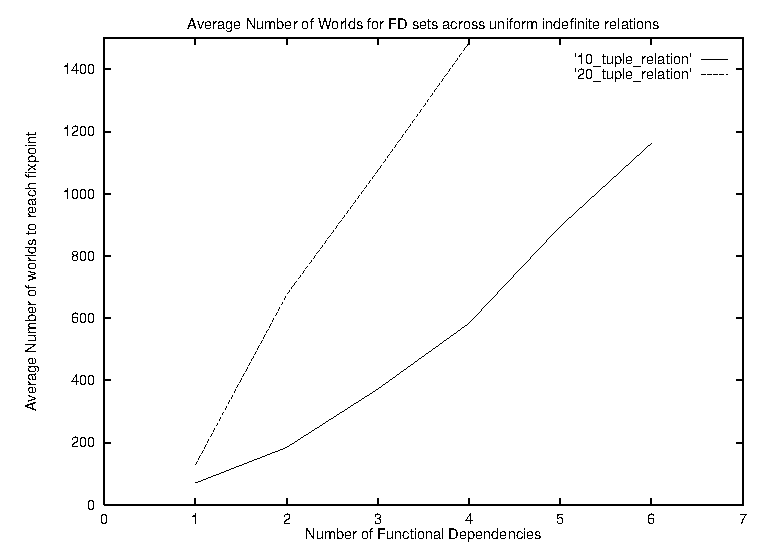
\includegraphics{../consistency/boot_mean1.eps}}}
\caption{\label{graph:linboot}\scriptsize{Average number of worlds to
reach an approximate fixpoint of the mean bootstrapped ND values in 10
and 20 tuple random relations}}
\end{figure}


\begin{definition}[The Bootstrap Standard Error for Indefinite Relations]
\begin{rm}
The sample \linebreak[4] standard error in the values for $B$ bootstrapped
values is:
\begin{displaymath}
\hat{se}_B = \{ \frac{1}{B}\Sigma_{i = 1}^{B}(\bar{s}(\tilde{p}^\star) - \bar{s}(\tilde{p}^\star_b)) \}^{1/2}
\end{displaymath}
\end{rm}
\end{definition}

We now describe the methods of our Bootstrap application, detailed in
Algorithm~\ref{alg:blimit}.
We start with a small initial sample size and a 
Bootstrap Replication Size $B$. 
Having created $B$ bootstrap samples we will have a bootstrap
mean of all values in the form of an ND set. For this value
we can use the bootstrap to calculate the standard deviation
(and other statistics if desired). From this we can empirically infer the width of the interval
in which a certain percentage of the relations occur. We continue
to increase the sample size by a fixed amount, $\delta$, until we reach 
a point where
the mean value of the NDs in the ND set converge. This 
provides a parameter whereupon anything higher is unlikely to have 
much additional change in variance. It is unlikely, even for an ND set with
just one dependency, for this to be reached randomly and running
our simulations in batches of 500 implied that any fixpoint values as 
outliers would have a negligible impact on the final results.

\medskip

We also examined the variance of the
observed possible worlds, for a range of original sample sizes,
 as the bootstrap replication
size was scaled from 20 up to 50,000 to decide on a suitable BRS. 
As this was increased we noted that
above 1000 there was negligible change in the variance. For the purposes
of our experiment setting B at 100 gave a suitable value
which allowed numerous repetitions of the complete bootstrapping process
in a reasonable time, knowing that there would be only a minimal change
in the variance for any increases. Additionally we experimented with 
using the original indefinite 
relation for each resampling iteration from which $n$ possible worlds are
sampled each time. The variance is much higher in this case as we
have all possible worlds to select from for each sample of size $n$.
In terms of reaching a fixpoint this takes much longer and was not used
in the final simulations. It could be of use
in situations where the
bootstrap sample may be unrepresentative of the population.


\subsection{Finding an approximate solution to the consistency problem}
\label{sec:consist_approx}

We focus on finding an approximation N of F for an indefinite relation
$r$ such that $r \weak$ N
using Algorithm~\ref{alg:check}, denoted by CHECK\_CONS($r$, F, $B$),
where $B$ is the bootstrap replication size (BRS).
Recall that we have assumed that $\mid r \mid = m+1$, where $m \ge 1$;
if $\mid r \mid < 2$, then $r \weak$ F trivially holds. 

\medskip

 Algorithm~\ref{alg:bstrap}, BOOTSTRAP($N_{bag}$,$s$,$B$),
describes the standard bootstrap procedure which returns the mean value
of ND sets for a number $B$ of Bootstrap replications, sample size $s$ and a
sample population $N_{bag}$ of ND sets. The value $\alpha$
provided by the bootstrap is used both in ND\_GEN and CHASE\_GEN.
 Algorithm~\ref{alg:blimit}, WORLD\_LIMIT($r$,$F$,$B$), implements our novel use 
of the Bootstrap procedure. We
base our procedure on the assumption that different sample sizes are
required according to the variance within an indefinite relation in
the different ND sets which may be satisfied in possible
worlds. The number of dependencies in the given FD set also influences
the results obtained from our use of the bootstrap. In Section~\ref{sol:res}
we show that this application of the bootstrap returns an upper bound on 
the number of worlds required for a good answer. Unlike many statistical
operations, the BOOTSTRAP
algorithm operates in exactly the same manner as a standard bootstrap
procedure despite the fact that we potentially have all possible worlds
within the indefinite relation.  Based on this we conducted experiments
whereby the bootstrap resamples were obtained not from the original
sample but from the indefinite relation. As stated, the variance of resampling
from the relation
was much higher than resampling from the sample and in such cases the upper bound was 
much higher.
Therefore we conjecture that it is suitable to use just one original sample
from the indefinite relation within each iteration of WORLD\_LIMIT.


{\line
\begin{figure}[ht]
\begin{center}
\fbox{\begin{minipage}[t]{16cm}
\begin{algorithm}[{\rm BOOTSTRAP}($nd\_bag$, $n$, $B$)]\label{alg:bstrap}
\begin{rm}
\begin{tabbing}
t1\=t2\=t3\=t4\=t5\=t6\=t7\=t8\=t9\=t10\= \kill \\
\ra. \>  {\bf begin} \\
\sa. \>  \>  ND\_mean := $\emptyset$ ;\\
\sa. \>  \> {\bf for }  1 to $B$ {\bf do }\\
\sa. \>  \> \> ND\_samp := Uniform Randomly select $n$ ND \\
\> \> \> \> \> \> \> \> sets from $nd\_bag$ with replacement; \\
\sa. \>  \> \> Insert the mean of ND\_samp into ND\_mean; \\
\sa. \>  \>  {\bf end for}\\
\sa. \>  \> {\bf return} the mean of ND\_mean; \\
\sa. \>  {\bf end.}
\end{tabbing}
\end{rm}
\end{algorithm}
\caption{\label{cp:fig:bootstrap} The Bootstrap procedure for
indefinite relations}
\end{minipage}}
\end{center}
\end{figure}
}


{\line
\begin{figure}[ht]
\begin{center}
\fbox{
\begin{minipage}[t]{16cm}
\begin{algorithm}[{\rm JACKKNIFE}($nd\_bag$)]\label{alg:jack}
\begin{rm}
\begin{tabbing}
t1\=t2\=t3\=t4\=t5\=t6\=t7\= \kill \\
\ra. \>  {\bf begin} \\
\sa. \>  \>  ND\_m := $\emptyset$;\\
\sa. \>  \>  $n$ := $\mid nd\_bag \mid$;\\
\sa. \>  \> {\bf for } $j$ := 1 to $n$ {\bf do }\\
\sa. \>  \> \> ND\_samp := $nd\_bag$ - $nd_j$; \\
\sa. \>  \> \> Insert the mean of ND\_samp into ND\_m; \\
\sa. \>  \>  {\bf end for}\\
\sa. \>  \> {\bf return} the mean of ND\_m; \\
\sa. \>  {\bf end.}
\end{tabbing}
\end{rm}
\end{algorithm}
\caption{\label{cp:fig:jackknife} The Jackknife procedure for
indefinite relations}
\end{minipage}}
\end{center}
\end{figure}
}





{\line
\begin{figure}[ht]
\begin{center}
\fbox{
\begin{minipage}[t]{10cm}
\begin{algorithm}[{\rm WORLD\_LIMIT }($r$, F, B)]\label{alg:blimit}
\begin{rm}
\begin{tabbing}
t1\=t2\=t3\=t4\=t5\=t6\=t7\= \kill \\
1.  \> \> {\bf begin} \\
2. \> \> \> $n$ := initial($r$); \% sample size \\
3. \> \> \> $\hat{N}_0$ := {\em Highest ND set possible in} $r$; \\
4. \> \> \> $\hat{N}_1$ := $\emptyset$; \\
5. \> \> \> $j$ := 1; \\
6. \> \> \> {\bf while} $\hat{N}_j,\hat{N}_{j-1}$ are not approx. fixpoint  {\bf do}  \\
7. \> \> \> \> ND\_bag := $n$ ND sets from $n$ possible worlds; \\
8. \> \> \> \> $\hat{N}_j$ := BOOTSTRAP(ND\_bag, $n$, B); \\
9. \> \> \> \> $n$ := $n + \delta$;  \% Increase the sample size by $\delta$ \\
10. \> \> \> \> $j$ := $j$ + 1;\\
11.   \> \> \>{\bf end while}\\
12. \> \> \> {\bf return} $n$;\\
13. \> \> {\bf end.}
\end{tabbing}
\end{rm}
\end{algorithm}
\caption{\label{cp:fig:world_limit} The WORLD\_LIMIT algorithm for
incremental bootstrap sampling in indefinite relations}
\end{minipage}}
\end{center}
\end{figure}
}



\subsection{The Chase and Hill-Climbing Algorithm}

Algorithm~\ref{alg:cp_ndchase}, CHASE($r$, N), is 
called within CHECK\_CONS. It is a heuristic procedure extended from the
standard chase procedure for FDs \cite{bv84,Mann92} which, given the
current set of NDs, attempts to remove extraneous or redundant information that
may be preventing the ND set from being satisfied. The forward chase removes extraneous values
from indefinite cells in attributes which are in the right hand
side of the given FD which is satisfied numerically but not functionally and 
therefore generalised to an ND.  Informally, a partition on attributes
in the left
hand side of the FD which has more elements than the branches of the ND is selected
and indefinite cell values of attributes in the right hand side of the
FDs whose appearance in a possible world would cause the ND to
be unsatisfied are removed. The backward chase removes values from
indefinite cells in attributes on the left hand side of the given
FDs which would have otherwise prevented satisfaction of the current
ND if that value had been selected for inclusion within a possible world.

\medskip

Algorithm~\ref{alg:check}, CHECK\_CONS($r$, F, $B$), uses the CHASE
procedures, generates a suitable sample size $\alpha$ using the bootstrap 
and then iterates $\alpha$ times from an initial possible world
generated by ND\_GEN the CHASE in a hill climbing fashion.
Algorithm~\ref{alg:gen}, ND\_GEN($r$, N, $\alpha$), invoked from
CHECK\_CONS, attempts to generate a definite relation using random
selection in conjunction with chase procedures. Using such random
selection in this manner allows for a value to be removed from an
indefinite cell which may then allow subsequent redundant values to be
removed by the chase procedure. 

Algorithm~\ref{alg:chase-gen}, CHASE\_GEN($r$, N, $\alpha$),
called from ND\_GEN, selects a partition within the relation for which
an ND is not satisfied and attempts to unify any two indefinite cells
which have at least one common value. This is repeated until no
further changes can be made. The empirical results of our simulations
show that using these heuristic algorithms generate, on average, equivalent
if not better, approximations in a much faster time.


Firstly, we present the algorithms used in our approach.
We find an approximation N of F such that $r \weak$ N
using the following algorithm, denoted by CHECK\_CONS($r$, F, $B$),
where $B$ is the bootstrap replication size.
Recall that we have assumed that $\mid r \mid = m+1$, where $m \ge 1$;
if $\mid r \mid < 2$, then $r \weak$ F trivially holds and we refer to
definition~\ref{def:covered}.

{\line
\begin{figure}[ht]
\fbox{\begin{minipage}{16cm}
\begin{algorithm}[{\rm CHECK\_CONS}($r$, {\rm F}, $B$)]\label{alg:check}
\begin{rm}
\begin{tabbing}
t1\=t2\=t3\=t4\=t5\=t6\=t7\= \kill \\
\ra.  \> \> {\bf begin} \\
\sa.  \> \> \> BOT := the bottom element of ${\cal L}_m$(F); \\
\sa.  \> \> \> $s$ := CHASE($r$, BOT); \\
\sa.  \> \> \> {\bf if} $s$ is undefined {\bf then} \\
\sa.  \> \> \> \> {\bf return} \{X $\to^{m+1}$ Y $\mid$ X $\to$ Y $\in$ F\}; \\
\sa.  \> \> \> {\bf end if}; \\
\sa.  \> \> \> APPROX := BOT; \\
\sa.  \> \> \> $\alpha$ := BOOTSTRAP\_CONS($r$,APPROX,{\rm F},$B$); \\
\sa.  \> \> \> S := $\emptyset$; \\
\sa.  \> \> \>  {\bf while} APPROX $\not=$ F and $\mid$S$\mid \le \alpha$ {\bf do} \\
\sa. \> \> \> \>  {\bf repeat} \\
\sa. \> \> \> \> \>  gen\_rel := ND\_GEN($s$, APPROX, $\alpha$); \\
\sa. \> \> \> \> \>  {\bf if} gen\_rel is not definite {\bf then} \\
\sa. \> \> \> \> \> \> {\bf return} APPROX; \\
\sa. \> \> \> \> \>  {\bf end if} \\
\sa. \> \> \> \>  {\bf until} gen\_rel $\not\in$ S; \\
\sa. \> \> \> \>  S := S $\cup$ \{gen\_rel\}; \\
\sa. \> \> \> \>  {\bf while} $\exists$ G such that APPROX $\cover$ G and gen\_rel $\models$ G {\bf do} \\
\sa. \> \> \> \> \>  APPROX := G;  \% hill climbing step \\
\sa. \> \> \> \>  {\bf end while} \\
\sa. \> \> \> \> {\bf if} $\exists$ G such that APPROX $\cover$ G and CHASE($s$, G) is defined {\bf then} \\
\sa. \> \> \> \> \> $s$ := CHASE($s$, G); \\
\sa. \> \> \> \> {\bf else} \\
\sa. \> \> \> \> \> {\bf return} APPROX; \\
\sa. \> \> \> \> {\bf end if} \\
\sa. \> \> \>  {\bf end while} \\
\sa. \> \> \> {\bf return} APPROX; \\
\sa. \> \> {\bf end.}
\end{tabbing}
\end{rm}
\end{algorithm}
\caption{\label{cp:fig:check_cons} The CHECK\_CONS algorithm for
approximating solutions to the consistency problem}
\end{minipage}}
\end{figure}
}
\medskip


The algorithm ND\_GEN($s$, N, $\beta$), which is invoked from CHECK\_CONS, 
is given below. Algorithm CHASE\_GEN($s$, N, $\gamma$),
which is invoked from ND\_GEN,
utilises the ND set N in order to assist ND\_GEN
to generate a definite relation that satisfies N. Algorithm ND\_CHASE is
called within CHECK\_CONS. It is a heuristic procedure extended from the
standard chase procedures for FDs \cite{bv84,Mann92} which, given the
current set of NDs, attempts to remove extraneous information that
may be preventing the ND set from being satisfied. Algorithm BOOTSTRAP
desribes the standard bootstrap procedure which return the mean value
of ND sets for a number $b$ of Bootstrap replications. The value $\alpha$
provided by the bootstrap is used both in ND\_GEN and CHASE\_GEN.

\medskip

 Algorithm
WORLD\_LIMIT describes our novel use of the Bootstrap procedure. We
base our procedure on the assumption that different sample sizes are
required according to the variance within an indefinite relation in
the different ND sets which may be satisfied in possible
worlds. The number of dependencies in the given FD set also influences
the results obtained from our use of the bootstrap. In section~\ref{sol:res}
we show that this application of the bootstrap returns an upper bound on 
the number of worlds required for a good answer. Unlike many statistical
operations, the BOOTSTRAP
algorithm operates in exactly the same manner as a standard bootstrap
procedure despite the fact that we potentially have all possible worlds
within the indefinite relation.  Based on this we conducted experiments
whereby the bootstrap resamples were obtained not from the original
sample but from the indefinite relation. The variance of this was much
higher than otherwise and in such cases the upper bound was much higher.
Therefore we conjecture that it is suitable to use just one original sample
from the indefinite relation within each iteration of WORLD\_LIMIT.


\medskip

\subsubsection{The Naive Algorithm}

We now briefly describe the naive version of CHECK\_CONS. This simply
generates a fixed number of possible worlds and returns the ND set with
the closest proximity to that of a set of FDs.
It is quite feasible to consider the use of the bootstrap in conjunction
with a naive approach though here we would require the generation of 
$\alpha$ definite worlds, exactly the upper bound returned from the
bootstrap, thereby increasing computation time. Use of the bootstrap
in a naive procedure is redundant given that such computation time
would be better spent generating new possible worlds and not
resampling.


{\line
\begin{figure}[ht]
\fbox{\begin{minipage}{16cm}
\begin{algorithm}[{\rm ND\_GEN}($s$, {\rm N}, $\beta$)]\label{alg:gen}
\begin{rm}
\begin{tabbing}
t1\=t2\=t3\=t4\=t5\=t6\=t7\= \kill \\
\ra.  \> \> {\bf begin} \\
\sa.  \> \> \> gen\_rel := CHASE\_GEN($s$, N, $\beta$); \\
\sa.  \> \> \> {\bf if} gen\_rel is undefined {\bf then} \\
\sa.  \> \> \> \> {\bf return} gen\_rel; \\
\sa.  \> \> \> {\bf end if} \\
\sa.  \> \> \> Fail := 0; \\
\sa.  \> \> \> {\bf while} gen\_rel is not definite and Fail $\le \beta$ {\bf do} \\
\sa.  \> \> \> \> Tmp := gen\_rel; \\
\sa.  \> \> \> \> Uniformly randomly reduce an indefinite cell in gen\_rel to one value; \\
\sa. \> \> \> \> gen\_rel := CHASE\_GEN(gen\_rel, N, $\beta$); \\
\sa. \> \> \> \> {\bf if} gen\_rel is undefined {\bf then} \\
\sa. \> \> \> \> \> gen\_rel := Tmp; \\
\sa. \> \> \> \> \> Fail := Fail + 1; \\
\sa. \> \> \> \> {\bf end if} \\
\sa. \> \> \> {\bf end while} \\
\sa. \> \> \> {\bf return} gen\_rel;  \\
\sa. \> \> {\bf end.}
\end{tabbing}
\end{rm}
\end{algorithm}
\caption{\label{cp:fig:nd_gen} The ND\_GEN algorithm for
generating a possible world}
\end{minipage}}
\end{figure}
}

{\line
\begin{figure}[ht]
\fbox{\begin{minipage}{16cm}
\begin{algorithm}[{\rm CHASE\_GEN}($s$, {\rm N}, $\gamma$)]\label{alg:chase-gen}
\begin{rm}
\begin{tabbing}
t1\=t2\=t3\=t4\=t5\=t6\=t7\= \kill \\
\ra.  \> \> {\bf begin} \\
\sa.  \> \> \> Result := $s$; \\
\sa.  \> \> \> Tmp := $\emptyset$; \\
\sa.  \> \> \> Fail := 0; \\
\sa.  \> \> \> {\bf while} Tmp $\not=$ Result {\bf do} \\
\sa.  \> \> \> \> Tmp := Result; \\
\sa.  \> \> \> \> {\bf if} $\exists$ X $\to^k$ Y $\in$ N, a partition $p$ on X in Result with $\mid p \mid \ge k + 1$ {\bf then} \\
\sa. \> \> \> \> \> Unify two values in rhs of partition {\bf or}\\
\sa.  \> \> \> \> \> {\bf if} Fail $\le \gamma$ {\bf then}\\
\sa.  \> \> \> \> \> \> Increment Fail {\bf and} Result := $s$, Tmp := $\emptyset$;\\
\sa.  \> \> \> \> \> {\bf else} \\
\sa.  \> \> \> \> \> \> Assign {\em undefined} to values in rhs of partition;\\
\sa.  \> \> \> \> \> \> {\bf return} Result;  \\
\sa. \> \> \> \> {\bf end if} \\
\sa. \> \> \> {\bf end while} \\
\sa. \> \> \> {\bf return} Result;  \\
\sa. \> \> {\bf end.}
\end{tabbing}
\end{rm}
\end{algorithm}
\caption{\label{cp:fig:chase_gen} The CHASE\_GEN algorithm for
applying a chase method randomly}
\end{minipage}}
\end{figure}
}
\medskip




\section{Simulations and Results}\label{sec:cpresults}
			\index{Bias|see{Changing Bias}}
			\index{Changing Bias}
	

We now discuss the simulations conducted to examine the 
viability of our methods for attempting to find a
consistent possible world within indefinite relations.
We concentrated on a few FD sets demarcated by the number of
dependencies in the set and whether they were BCNF or non-BCNF. 
In Table~\ref{table:simpar} we present an overview of the parameter
ranges for the simulations
conducted. Batches containing 500 runs were conducted so that we 
could find reliable averages. The range of possible inputs for an indefinite
relation is very large. We limited the size of our relations to 50 tuples,
and carried out the simulations with batches having a maximum indefinite
cell arity of up to six elements and a domain size for each attribute of
up to 10 elements, noting that the domain size must be higher than the
maximum indefinite cell arity.  The weighting of the likelihood of the
presence of an indefinite cell was also varied for selected batches.
In a {\em standard} batch we randomly generate a relation wherein each
cell has a 50\% chance of being indefinite. If it is selected to be
indefinite then its arity, up to the maximum for the batch, is then
randomly selected. The weighting was varied in batches for suitable
FD sets from 25\% to 75\% likelihood of being indefinite on the
attributes according to whether they are in the left or right hand side
of an FD.

{\line
\begin{table}[ht]
\begin{center}
\begin{tabular}{|l||l|}
\hline
{\bf Number of FD sets}  & 12 \\ \hline
{\bf Program Versions} & Naive/Chase and hill-climbing \\ \hline
{\bf Single FD simulations} & 1 batch for each domain/tuple/cell-arity combination\\ \hline
{\bf Batch Range} & 500 runs in each \\ \hline
{\bf Domain Range} & 1 - 10  \\ \hline
{\bf Tuple Range} & 5 - 50  \\ \hline 
{\bf Cell-Arity Range} & 2 - 6 (domain size $\ge$ cell-arity) \\ \hline 
\end{tabular}
\end{center}
\caption{\label{table:simpar} Simulation details }
\end{table}
}



\subsection{Results}\label{sol:res}

We now present some results based upon our simulations. We show
in Figure~\ref{graph:4.1} results depicting the closest proximity
within a batch for 
both the naive and the chase and hill-climbing approaches for the
FD set $F_1 = \{A \to B, A \to C, A \to D \}$ having a domain of 7 and 
containing indefinite cells of a maximum arity 6.  The limit, $\alpha$,  
on the iteration size, as supplied by the Bootstrap was 
equalled in less than 1\% of the simulations, showing this to
be a suitable upper bound.

\begin{figure}
\centerline{\scalebox{0.7}{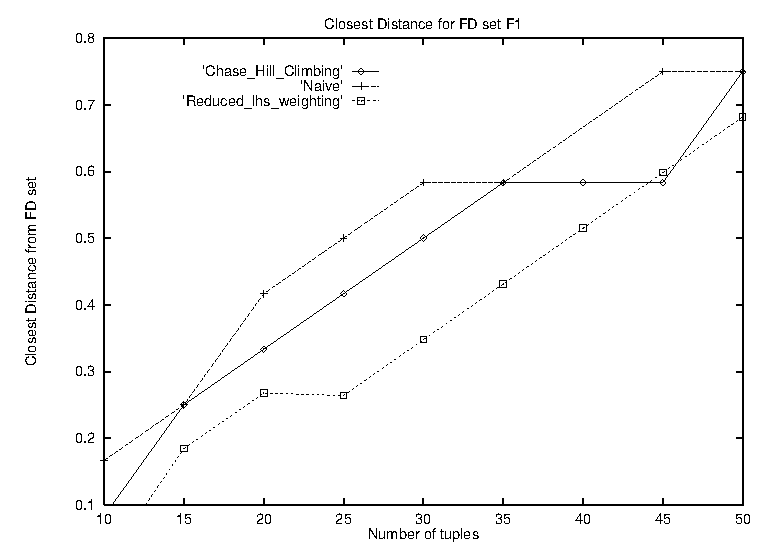
\includegraphics{../consistency/f1_result.eps}}}
\caption{\label{graph:4.1}\scriptsize{Closest Proximity for FD set $F_1$ across a number of different weighted relations}}
\end{figure}

\smallskip

\subsection{Analysis of the Chase results}

Simulations showed that the chase 
procedure outperformed
the naive approach, on average, by an increasing margin as the number of
tuples within a randomly generated relation increased. This margin became
slightly larger at higher domain sizes within relations. Obviously, as the
tuple and domain size are increased, the chase procedure becomes more 
effective due to the increased probability of their being more redundant 
values to remove. We can see in Figure~\ref{graph:4.1}
that if there is a bias towards having more indefinite cells in attributes
which are present in the right hand side of functional dependencies then
the average proximity for both the naive and chase approaches are better
than an even weighting, with the chase procedure outperforming the naive
at an earlier stage. An increased number of indefinite cells in attributes
on the right hand side of FDs implies that there may be more values which
may lead to unnecessarily low ND satisfaction (i.e. each ND will have a 
larger branching factor) which can now be removed by the chase heuristic.
Our simulations show the increased efficacy of the chase in such cases.
A larger indefinite cell arity also implies that the chase will have more
values to remove and therefore perform even better. In the case of reducing
the weighting of indefinite cells of the left hand side of FDs, a naive
approach performs much worse than in an evenly weighted relation due to
there being fewer indefinite cells from which it can select different
values, thereby preventing much variation of the partitioning on the NDs 
in a relation which might otherwise occur. We did not find a
significant difference between using BCNF and non-BCNF FD sets.

Figure~\ref{graph:4.2} shows results for
$F_3$ = $F_1 \cup \{ BD \to A \}$. For this relation
the chase procedure performs poorly with respect to the naive technique
on average. We believe this is due to the interference of the attributes
within the FD set having attributes determining and being determined by
each other which reduces the application of the chase heuristic.
 We note however that the best results within a batch obtained by both
the naive and the chase and hill climbing are increasingly similar as
relation size increases. Also, the chase and hill climbing approach requires
far fewer worlds.

\begin{figure}
\centerline{\scalebox{0.7}{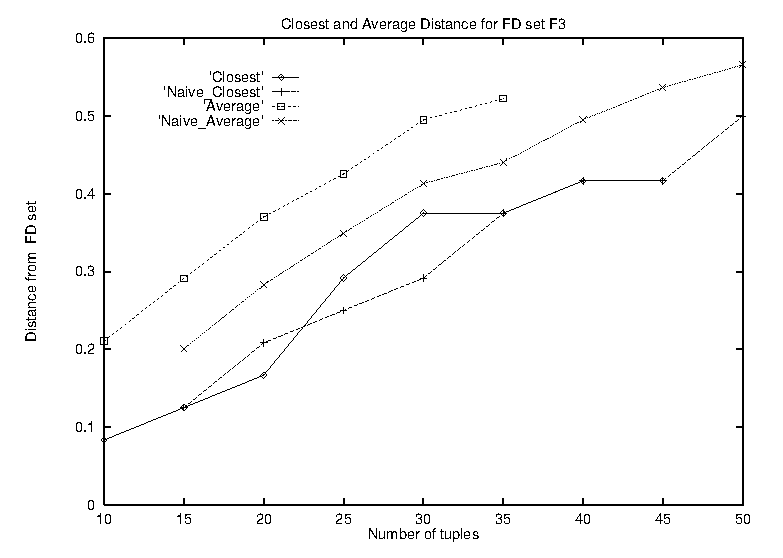
\includegraphics{../consistency/f3_result.eps}}}
\caption{\label{graph:4.2}\scriptsize{Closest and Average Proximity for FD set $F_3$  }}
\end{figure}

\begin{figure}
\centerline{\scalebox{0.7}{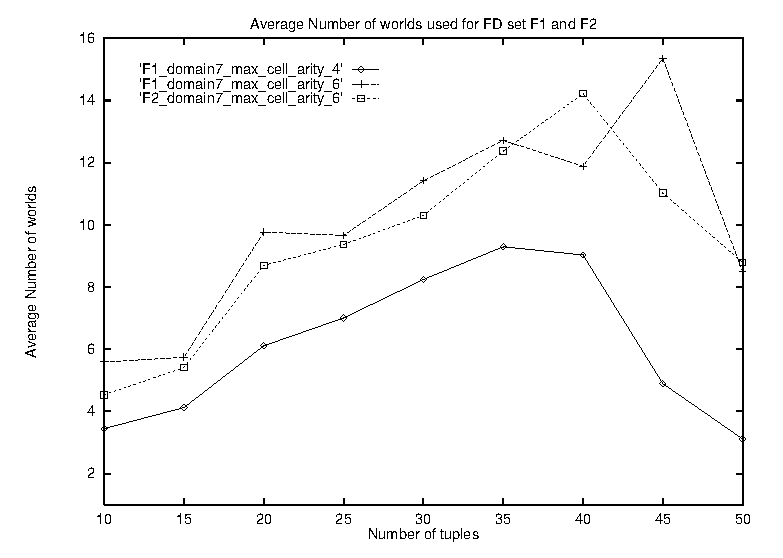
\includegraphics{../consistency/worlds2.eps}}}
\caption{\label{graph:4.3}\scriptsize{ Average Number of Worlds required by
the chase and hill-climbing approach}}
\end{figure}

In Figure~\ref{graph:4.3} we see that, for both FD set $F_1$ and 
$F_2 = \{ A \to B, B \to C, C \to D \}$, as the number of tuples
increases there is a slight peak, after which further increases in the number
of tuples results in a fall in the average number of worlds required.
This is based on every relation within a batch having a fixed domain
size $d$ and an indefinite cell maximum arity, reaching a point where it is
likely that any further increases in the tuple size will lead to the
satisfaction of the numerical dependency set with each branch determining
up to $d$ branches and so fewer worlds are required before any 
attempts to apply the chase returns an undefined relation implying that
nothing better can be found. The peaks in Figure~\ref{graph:4.3} were reflected in the values
of $\alpha$ returned by our bootstrap technique. In our
application of the bootstrap, as the relation size of a random relation 
is increased and the domain size is held constant, the sampling will also
reach a point where the variance in the samples amongst the randomly
generated possible worlds is reduced due to most possible worlds 
satisfying the NDs each with a branching factor close to their domain
size.  The bootstrap in conjunction 
with a naive approach is not really feasible based on it simply being
a very large naive generation of possible worlds. The superiority of
the chase and hill-climbing
procedure in dependency sets which do not determine each other highlighted
this fact.


\subsection{Real-World Applications and Examples}\label{sec:apps}
 
In \cite{inv91} we are shown how indefinite information may be used to
represent a possible schedule. Our approach allows us to discover an
approximation to an {\em ideal} relation, {\em ideal} being a relation
which satisfies
a set of FDs. NDs are a useful tool in this context and indeed 
schedule representation within relational databases would be enhanced with
their use. Any approximation
provided by our system for a relation can be analysed by the system
users. The schedule which is produced by this, or any other, system can
be studied with respect to the result of our procedures. If there are
FDs which are not satisfied within the relation and these are less
functional than those provided as output by our chase and hill-climbing
approach we can assume a superior schedule exists. The Bootstrap
parameters will also tell the user valuable information on the
variance and mean of the possible dependency sets which will enhance
their knowledge of the indefinate data within the relation.

\medskip
 
NDs, together with the metric presented in section~\ref{sec:consist_approx} are applicable
within any relational database for approximating and comparison of FD sets.
In a data mining environ this could be used for contrasting approximations
in relations over the same attributes which may be in use at different
locations.


\subsection{Relational Data Sets utilised}

\subsection{Statistics for Assessing the Data Sample}

\subsection{Changing Bias of indefinite
information}\label{subsec:cp_bias}

We now briefly discuss differences within resampling for relations
with different bias of indefinite cells in the relation. Experiments
showed that relations with different ND set satisfaction with the
definite cells in an indefinite relation have different variances
from a smaller range when the NDs are satisfied less functionally to a
larger variance when the NDs satisfied are close to FDs. This is
explained due to the definite cells themselves being further from or
closer to FD set satisfaction which implies, respectively, a smaller
or larger change in proximity within the possible worlds.

\smallskip

In Figure~\ref{graph:cp_hist1} we provide a histogrom of
2000 bootstrap replications for a relation with 20 tuples, a
definite lhs and a right hand side with 50\% of tuples indefinite.
We emphasise that more indefinite cells on the left hand side of the
FDs decrease the variance due to each lhs indefinite value creating
new partitions on attributes in the lhs whilst more indefinite cells
on the rhs of FDs increase the variance. Obviously, the arity of
indefinite cells and intersections of values temper the change in
variance. 


\begin{figure}
\centerline{\scalebox{0.6}{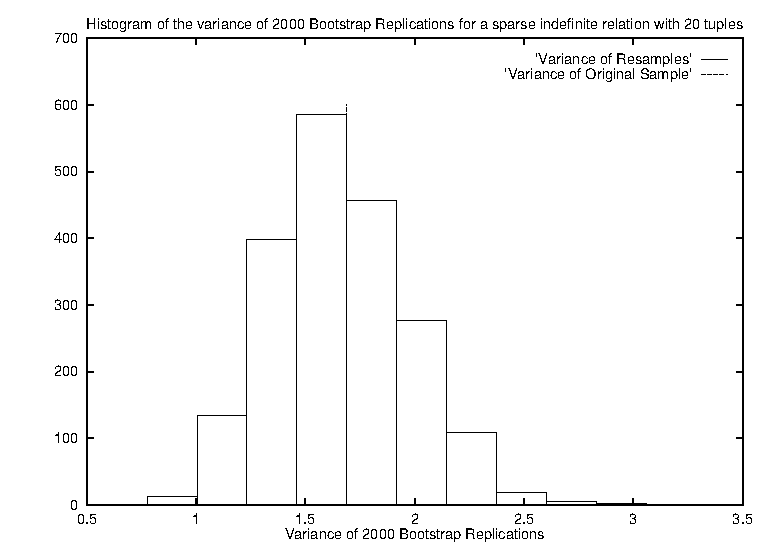
\includegraphics{../consistency/var2000rel6w25.eps}}}
\caption{\label{graph:cp_hist1}\scriptsize{Histogram of 2000 bootstrap replications of sample size 25 for a 20 tuple relation, with a definite lhs and a
right hand side sparse in indefinite cells, otherwise the same}}
\end{figure}

\subsection{Similarity Results for ND sets}

\subsection{Finding a suitable sample size}

Our use of the bootstrap procedure was found to provide a suitable
upper bound on the number of worlds required by our algorithms. We
have explained how the dynamic resampling relies on the variance of ND
set satisfaction amongst possible worlds in the sample to infer when a
larger sample is not required.  The fact that this provided an upper
bound for our algorithms justifies its use. 
As the sample size grows, highlighted in
Figure~\ref{graph:conlim}, there is a reduction in variance between
previous iterations. The non-parametric nature of the resampling is
shown to be useful in that the empirical confidence limits for
the bootstrap process are
shown to converge for the distance measure of an ND set.


\begin{figure}
\centerline{\scalebox{0.7}{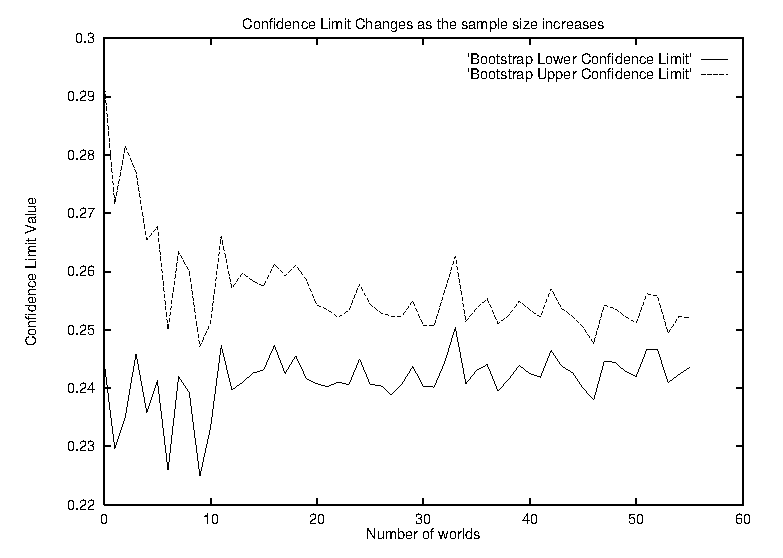
\includegraphics{../Bootstrap/efronlimit60.eps}}}
\caption{\label{graph:conlim}\scriptsize{Efron's empirical percentile
 confidence limits shown to converge for the distance measure of ND sets}}
\end{figure}


A problem with the bootstrap is also discussed in \cite{de83}. It
seems to occur when there is very little variation in the range
of values in the sample data. For instance, it may be the case that
we have an indefinite relation which for a given FD set is such that
nearly all possible worlds satisfy this FD set. Bootstrap sampling
on this data set would be judged to have a very high accuracy,
based on the empirical lack of variation found in the samples.
\cite{de83} says this would be incorrect. The bootstrap will always
perform badly when there is an indefinite relation
with only one or few worlds which we consider to be {\em good} in
the context of approximating FD sets.
Indeed, we do not say that the bootstrap performs badly, it merely
creates an average of the branching values based upon sampling with
replacement from the original subsample. This will always be a good
reflection of the average branching values in the ND set unless the
original $n$ samples are not a good reflection of the true values
in the relation.

Note that the bootstrap procedure can not be used to provide any
indication as to whether there is, or is not, present a very good
approximation to an FD set, or an FD set itself within the relation.
It will only provide an indication of this when there are a large 
number of very good FD sets. Therefore we can state:
\begin{enumerate}
\item If the values of the Bootstrap when a fixpoint is reached
are functional or near functional then the majority of possible
worlds will satisfy the dependency set functionally or nearly functionally.
\item If the values of the Bootstrap are not
nearly functional in proportion to the size of the relation this
indicates that most of the definite worlds are poor in terms of
satisfying the specified FD set nearly functionally
\end{enumerate} 

We can see from this that the Bootstrap is an averaging mechanism.

\subsection{A Comparison with Jackknife Resampling}


The strategy of the jackknife is to remove a single data point from each
resample. This allows the creation of $n$ jackknife resamples from an
original sample of size $n$.  The bootstrap provides additional flexibility
in that the sample is made up of any values uniformly and randomly selected
with replacement from the original and, additionally, is not limited to
$n$ resamples.  In our process the number of worlds required is increased
until a fixpoint is reached. Using the jackknife as the worlds reach a
large number $q$ we are constrained to $q$ resamples, each of size $q-1$.
Under the bootstrap application we have a fixed number of resamples which,
in the majority of cases,
will increase to a sample size that is smaller than the $q$ required by the 
jackknife. We found
that the results were very similar for both the bootstrap and jackknife, 
highlighted in Figure~\ref{graph:bj1}, 
despite our use of the bootstrap conducting fewer replications than the
jackknife at large sample sizes. Based on the dynamic nature of our
resampling often requiring large sample sizes it is therefore much
more efficient to use bootstrap and not jackknife resampling. 
Figure~\ref{graph:bj1} also presents
the falling limit of the fixpoint as the domain size is held constant but
the tuple size increases. 
\begin{figure}
\centerline{\scalebox{0.7}{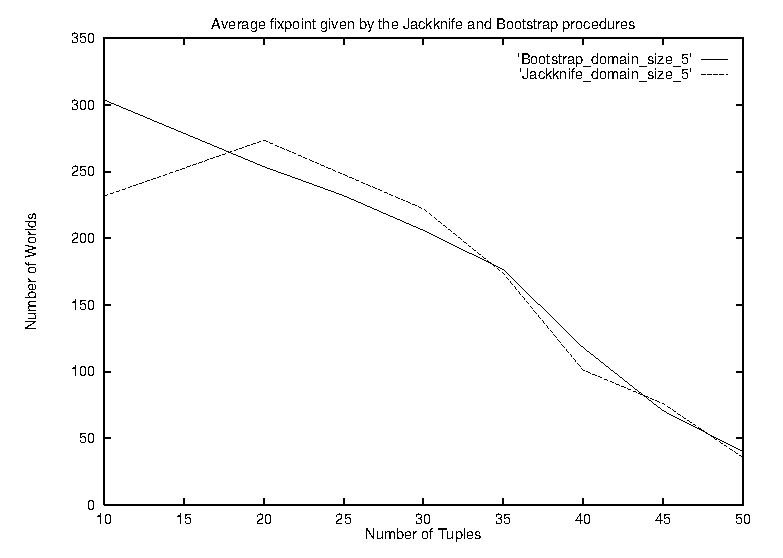
\includegraphics{../Bootstrap/bootjackav.eps}}}
\caption{\label{graph:bj1}\scriptsize{ Average Number of Worlds given as 
upper bounds by the Bootstrap and Jackknife techniques}}
\end{figure}



\section{Discussion}\label{sec:cp_disc}


We have described how the representation of indefinite information is a 
valuable extension to relational databases, following on from the work
in \cite{inv91,vn95}. In addition to this we 
note that NDs suitably generalise FDs
both in a database design context where they may be used in their
own right when an FD is too strict \cite{gm85b}, or within the context of their
usage in this paper where we have used them to approximate FDs based
on all possible NDs which may hold within a relation for a given set of FDs forming a complete lattice.  The use of NDs extends the work of \cite{vn95}
where relations which do not satisfy the constraint set functionally are
said to be {\em unrealizable}. In many dependency data mining applications,
which range from data summarisation to learning within decision trees \cite{psm93}, we may wish to obtain a numerical value, between 0 and 1, denoting how close a set of 
FDs are to being satisfied; the metric presented in this paper achieves
this. 
The consistency problem for relations with indefinite information is
widely known to be {\em NP-complete}. Therefore we cannot expect to
develop a polynomial time based solution unless $P = NP$ or the database is
restricted as in \cite{vn95}. Our approach
does however introduce an interesting new technique based on sampling,
extending the bootstrap to providing useful approximations for
problems such as the consistency problem. Essentially, it is based on
extracting a representative sample and inducing assumptions on the 
complete indefinite relation based on the variance within the samples, and
subsequently the Bootstrap resamples. We have shown this to provide us
with valid upper bounds.

\medskip

The simulations have shown that our procedure can provide useful
approximations to FD sets in the form of ND sets for any indefinite
relation. We compared different weightings of indefinite information within
a relation and showed that as a relation approaches what \cite{vn95}
refer to as a {\em good database}, one without indefinite information
in the left hand side of the dependencies, then the chase procedure for
NDs becomes more effective.The efficacy of the chase heuristic, extended in
this work to apply to NDs, over naive methods is shown in the
best result achieved within a batch. Also, on average around 10\% of 
the worlds used in 
a naive approach are required by a chase and hill-climbing approach.
The bootstrap provides a suitable upper bound with, on average, 
less than 1\% percent of relations generating the number of worlds it
takes to reach a fixpoint when using chase and the hill-climbing technique.
We are also planning to explore applications of NDs and bootstrap
applications within the temporal database domain, another area where
there is a combinatorial explosion of data points.

\medskip
\index{NP-Complete}
\index{Phase Transition}
A greater understanding of the behaviour of NP-complete problems
is provided in \cite{slm92,msl92}.  \cite{ckt91} introduces
the details of {\em phase transitions} occuring where NP-complete
problems become really hard.  These areas are dense in local
minima so that there are many near solutions which the search procedure
follows.  On either side of this critical boundary the 
problem distribution tends to be either over- or under- constrained.
For both of these cases the search is cut off quickly and the 
probability of success tends to 1 and 0 respectively. Phase
transitions  occur from a region where
most problems are easy and soluble to a region where most are
easy but insoluble. However, as \cite{sg94} note, there are
certain {\em exceptionally} hard problems on either side
of the phase transition which are much harder than those occurring
inside the phase transition. A study of these exceptionally
hard problems shows that they are the ones most likely to
encounter an insoluble subproblem at an early stage. \cite{ckt91}
points out that complex systems with many
interacting values can often be understood at the
macroscopic level which characterise the whole system.
We should seek, similarly, 
to understand where such transitions occur for the consistency
problem in further work, as they might provide a useful insight into
the representation of indefinite information in relations such as
suitable frequency of indefinacy.


